%%
%% Introdução
%%
\chapter{Introdução}
\label{introducao}

O crescimento tecnológico ocorrido nas últimas décadas constitui fator essencial e decisivo para o desenvolvimento de distintas áreas do conhecimento. O compartilhamento de informações mediante ambientes computacionais tem aumentado de maneira exponencial, visto que a vasta maioria das empresas consolidadas no mercado, independente da área de atuação, utilizam de sistemas de informação e redes de computadores para controle de seus respectivos negócios \cite{machado2005}.

Nesse contexto, onde informações restritas e confidenciais são compartilhadas em redes ao redor do mundo, o número de criminosos digitais (crackers) aumentou fortemente  \cite{nakamura2002}, o que pode ser observado na Figura \ref{fig:cert}. Assim como na sociedade, a segurança é marcada por uma evolução contínua e cíclica. A medida que novas modalidades de crimes são concebidas, em contrapartida, medidas para combater esses crimes são desenvolvidas. Além disso, os novos crimes sempre terão como alvo pontos pouco policiados ou vulnerabilidades do ambiente computacional, no caso do mundo digital \cite{nakamura2002}. Neste contexto, os ataques às redes de computadores, visando a captura de informações privilegiadas, se tornaram comuns e a diversidade dos ataques gerou a necessidade de investimento financeiro e intelectual na segurança de redes de computadores.

\begin{figure}[ht]
    \centering
    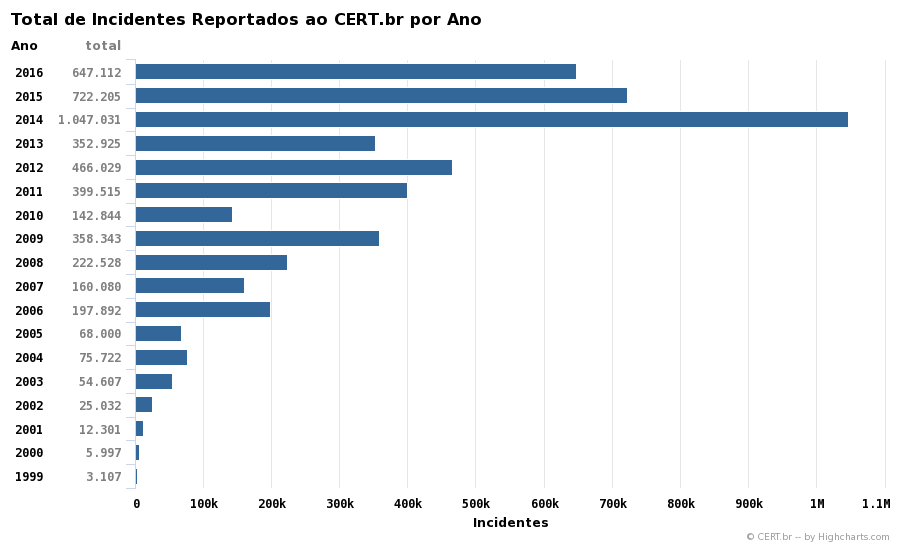
\includegraphics[scale=0.5]{Cap1/cert.png}
    \caption{Incidentes de segurança reportados ao CERT. Fonte: www.cert.br}
    \label{fig:cert}
\end{figure}


Dentre os modos mais comuns para a detecção e proteção contra invasões citam-se os Sistemas de Detecção de Intrusão (SDI), os quais atuam auxiliados por mecanismos de monitoramento de redes de computadores, com a finalidade de identificar ações que possam comprometer a integridade, confidencialidade ou disponibilidade de recursos \cite{crosbie1995} e aplicar medidas de correção de violações ocorridas. 

Entre os métodos usados na detecção de intrusão em redes, as estratégias adotadas são diversas, podendo utilizar sistemas especialistas, redes neurais artificiais, mineração de dados, agentes móveis, sistemas imunológicos artificiais (SIA), entre outros \cite{machado2005,delima2005,sujatha2012,hashemi2013,paiva2011}.

A aplicação de técnicas de inteligência artificial voltada à segurança computacional tem sido muito explorada nos últimos anos, com o objetivo de otimizar os métodos convencionais de detecção.

\section{Proposta}

\section{Estrutura do Trabalho}

\begin{comment}

https://www.quora.com/Why-is-it-better-to-use-Softmax-function-than-sigmoid-function


Why Use a One Hot Encoding?

A one hot encoding allows the representation of categorical data to be more expressive.

Many machine learning algorithms cannot work with categorical data directly. The categories must be converted into numbers. This is required for both input and output variables that are categorical.

We could use an integer encoding directly, rescaled where needed. This may work for problems where there is a natural ordinal relationship between the categories, and in turn the integer values, such as labels for temperature ‘cold’, warm’, and ‘hot’.

There may be problems when there is no ordinal relationship and allowing the representation to lean on any such relationship might be damaging to learning to solve the problem. An example might be the labels ‘dog’ and ‘cat’

In these cases, we would like to give the network more expressive power to learn a probability-like number for each possible label value. This can help in both making the problem easier for the network to model. When a one hot encoding is used for the output variable, it may offer a more nuanced set of predictions than a single label.


# SMOTE proposes several variants by identifying specific samples to consider
# during the resampling. The borderline version will detect which point to
# select which are in the border between two classes.

\end{comment}